% !TeX root = ../main.tex

\chapter{Standard Model}



The Standard Model (SM) is the theory used to describe the interactions between fundamental particles 
(which are listed in table~\ref{table:pdg-table}).
As far as we know, the interactions between fundamental particles are just four: \textit{Gravitational}, 
\textit{Electromagnetic}, \textit{Weak} and \textit{Strong}.
The SM is a non-Abelian Gauge theory whose symmetry group is:

\begin{equation}
    SU(3) \times SU(2) \times U(1)
\end{equation}

In reality this statement is unprecise, since what we know is only the Lie algebra of the SM.%
\footnote{
    An introduction to Group Theory is beyond the scope of this brief introduction to the SM, 
    but to not leave the reader completely dissatisfied with this statement, 
    what I will limit myself to say is that different groups share the same algebra, so having access only 
    to the algebra, we cannot uniquely determine the underlying group.}

This theory consists of two main sectors: Quantum Chromodynamics (QCD), which describes the Strong interaction 
and is based on the $SU(3)$ symmetry, and the Electroweak sector (EW), which desccribes the Weak 
and Electromagnetic interactions and is based on the $SU(2) \times U(1)$ symmetry.\\
The SM does not offer a proper description of \textit{Gravity}, it only suggests the existence of 
the \textit{Graviton}, the mediator of the gravitational interaction.
However, this particle has not been discovered thus far,  therefore a completely satisfactory quantum 
theory of gravity has yet to be formulated.\\

\begin{table}[h]
    \centering
    \begin{tabular}{ccccc}
    \toprule
    & Particle & Mass (MeV) & Mean Life (s) & Charge (e) \\
    \midrule
    \multirow{4}{*}{Leptons} & $e^-$ & $0.511 \pm 10^{-9}$ & $> 6.6 \times 10^{28}$ yr &  \\
    & $\mu^-$ & $105.7 \pm 10^{-6}$ & $2.197 \times 10^{-6}$ & $-1$  \\
    & $\tau^-$ & $1776.86 \pm 0.12$ & $(290.3 \pm 0.5) \times 10^{-15}$ &  \\
    & $\nu_e, \nu_{\mu}, \nu_{\tau}$ & $< 2 \times 10^{-6}$ & - & $0$  \\
    \midrule
    \multirow{6}{*}{Quarks} & $u$ & $2.16^{+0.49}_{-0.26}$ & - &   \\
    & $c$ & $(1.27 \pm 0.02) \times 10^3$ & - & $\frac{2}{3}$  \\
    & $t$ & $172.69 \pm 0.30 \times 10^3$ & - &   \\
    & $d$ & $4.67^{+0.48}_{-0.17}$ & - &    \\
    & $s$ & $93.4^{+8.6}_{-3.4}$ & - & $-\frac{1}{3}$  \\
    & $b$ & $(4.18^{+0.03}_{-0.02}) \times 10^3$ & - &   \\
    \midrule
    & Particle & Mass (GeV) & Decay Width (GeV) & Charge (e) \\
    \midrule
    \multirow{5}{*}{Bosons} & $\gamma$ & $< 10^{-24}$ & Stable & $< 10^{-35}$  \\
    & $W^{\pm}$ & $80.379 \pm 0.012$ & $2.197 \times 10^{-6}$ & $\pm 1$  \\
    & $Z^0$ & $91.1876 \pm 0.0021$ & $2.4952 \pm 0.0023$ & $0$  \\
    & $g$ & $0$ & - & $0$  \\
    & $H$ & $125.18 \pm 0.16$ & $< 0.013$ & $0$  \\
    \bottomrule
    \end{tabular}
    \caption{Properties of the Standard Model Particles as given by the PDG~\cite{pdg}.}
    \label{table:pdg-table}
\end{table}


As part of this introduction to the SM, before delving into the description and deduction of the main 
two sectors of the SM, I believe it is instructive to introduce the lagrangian of the SM.

\begin{equation}
    \mathcal{L}_{SM} = \mathcal{L}_{gauge} + \mathcal{L}_{Higgs} + \mathcal{L}_{Yukawa}
\end{equation}


\section{Electroweak Sector}

The Electroweak sector is the result of the unification of the Weak and Electromagnetic interaction and it 
is described by the symmetry group:

\begin{equation}
    SU(2)_L \times U(1)_Y
\end{equation}

This group has exactly four generators, one for each gauge boson (Z, $\gamma$, $W^{\pm}$).
The subscript “L" refers to the fact that only the left-handed component of particles interact weakly, 
whereas the right-handed component is non sensible to the Weak interaction.
The subscript “Y" indicates the Hypercharge.

Since only left-handed components interact weakly we put them in SU(2) doublet, whereas the right-handed
are put in a sterile SU(2) singlet:

\begin{align}
    \ell_L = 
    \begin{pmatrix}
    \nu_L\\
    e_L \\
    \end{pmatrix}
    \qquad
    e_R
\label{eq:lh}
\end{align}

The equation \ref{eq:lh} shows one lepton flavour, but can be extended to all three lepton flavours by 
adding an index “i".

Since the Weak interaction is chiral (only the left-handed particles interact weakly)
As a stepping stone to build the EW lagrangian we take in consideration the Dirac massless lagrangian:

\begin{equation}
    \mathcal{L} = \bar{\psi} i \slashed{\partial} \psi
\end{equation}
Requiring the invariance under $SU(2)_L \times U(1)_Y$ of the Dirac massless lagrangian:

To build the lagrangian of the EW sector we take the Dirac massless lagrangian 



\section{Quantum Chromodynamics}

\begin{figure}[h]
    \centering
    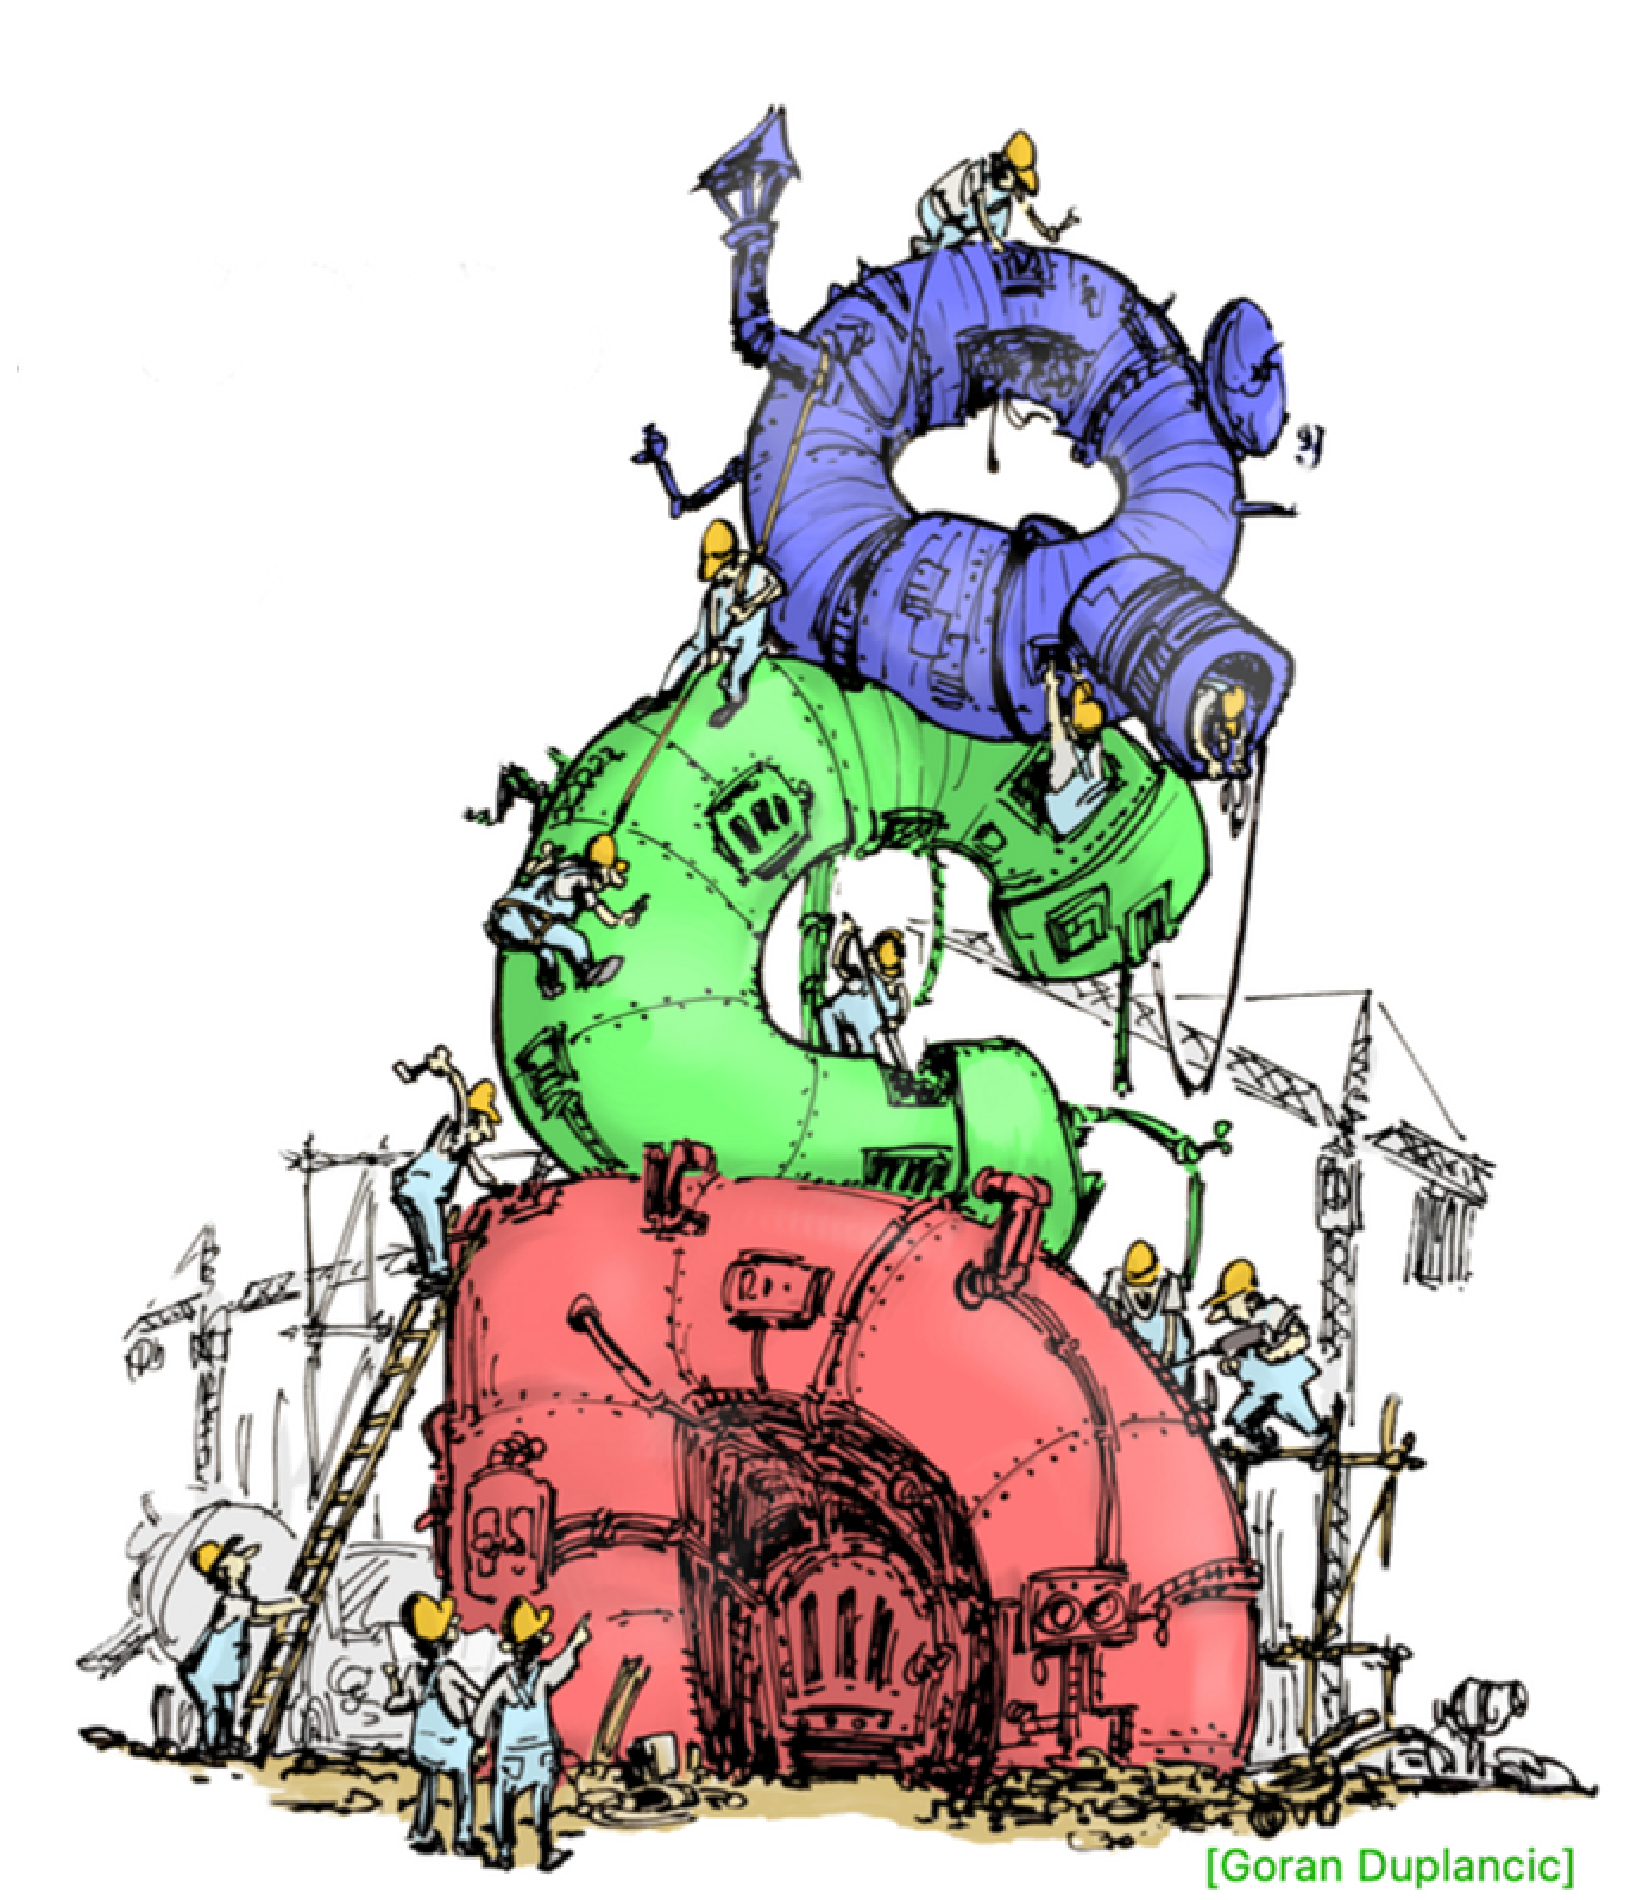
\includegraphics[scale=0.25]{sections/Chapters/Chapter1/Images/qcd.pdf}
    \caption{QCD is a colorful theory.}
\end{figure}

The QCD lagrangian is invariant under SU(3) color symmetry.

\begin{equation}
    \mathcal{L}_{QCD} = - \frac{1}{4} \sum_{a=1}^{8} F^a_{\mu \nu}F^{a \nu \mu} + \sum_{f=1}^{6} \overbar{\psi}_f^i
    (i \gamma^{\mu} (D_{\mu})_{ij} - m_f \delta_{ij}) \psi_f^j
\end{equation}

Let's discuss the indeces: $\mu$, $\nu$ are the usual Lorentz's indeces, $a$ is the gluon index, $f$ is the
flavour index, $i$ and $j$ are color indeces ($i$, $j = 1, 2, 3$).
Furthermore the lagrangian contains the Faraday's tensor and the covariant derivative:

\begin{align}
    &F^a_{\mu \nu} = \partial_{\nu} G^a_{\mu} - \partial_{\mu} G^a_{\nu} + g f^{abc}G_{\mu}^{b}G^c_{\nu} \\
    &(D_{\mu})_{ij} = \partial_{\mu} \delta_{ij} - i g \tau^a_{ij} G^a_{\mu}
\end{align}

where $f^{abc}$ are the structure's constant of the SU(3) group, $G^a_{\mu}$ is the gluon four-vector, 
$\tau^a$ are the SU(3) generators.

The main difference between the Strong and EW sector is that the spontaneous symmetry breaking 
mechanism is not necessary to describe quarks' masses, because the lagrangian's mass term is invariant 
under SU(3) symmetry.

\subsection{Parton Model}


\subsection{Jets}

When studying high-energy collisions one often has to consider processes with gluons and quarks in the final state.
Quarks and gluons can be produced in numerous processes such as the decay of W, Z and H bosons.
However, these high-energy quarks and gluons are not directly observed in the final state of the collision.
They tend to undergo successive branchings at small angles, producing a series of collimated quarks and gluons. 
This cloud of collimated particle is often referred to as “parton shower".
The fact that this parton shower is collimated traces back to the collinear divergence of QCD.
Starting from a parton with high virtuality (of the order of the hard scale of the process), 
the parton shower will produce branchings into further partons of decreasing virtuality, 
until one reaches a non-perturbative (hadronisation) scale, typically of order $\Lambda_{QCD}$ ($\sim$ 1 GeV).
At this stage, due to confinement, these quarks and gluons will form hadrons.
Conceptually jets are collimated flows of hadrons.

\subsection{Jet algorithms}

After discussing the meaning and origin of jets in the introduction, we require an infrared-safe definition of 
jets. Historically, the first definition of a process with two jets was given by Sterman and Weinberg. 
They defined a process with two jets as a process in which it is possible to identify two cones of angle $\delta$, 
within which all the energy of the process is contained, with a discrepancy of at most $\epsilon$.
The Sterman-Weinberg's cross section has two equivalent definitions:

\begin{align}
    \sigma_{SW} &= \sigma^{q \bar{q}} + \sigma^{3 partons}(E_i < \epsilon \sqrt{s} \land \theta_{ij} < \delta) + \\
    + \sigma^{4 partons}(E_i < \epsilon \sqrt{s} \land \theta_{ij} < \delta) + ... \\
    &= \sigma^{tot} - \int_{R} \frac{\sigma^{tot}}{d x_1 d x_2}
\end{align}


The first definition defines the SW cross section as the sum of the cross sections with an increasing number 
of partons in the partonic final state. The cross section with two partons does not require any constraints 
since it naturally produces two jets. The cross section with three partons, in order to have two jets in the 
final state, requires constraints on the third parton, which must not form a jet. Hence, it must be either 
inside one of the cones ($\theta_{ij} < \delta$) or have an energy below the tolerance of $\epsilon \sqrt{s}$. 
Similarly, the cross section with four partons has the same constraints but on two partons instead of just one.

The second equivalent definition defines the SW cross section as the whole cross-section minus the hard 
cross-section.
The integration domain $R$ identifies the hard region of the Dalitz plot (i.e., the central one).


In the modern era the jet definitions are \textbf{jet algorithms} which are well-defined procedure that tells 
how to reconstruct the jets from the set of hadrons in the final state of the collision.
A jet algorithm has three main building blocks:

\begin{itemize}
    \item \textbf{Distance}.\\
    The distance expresses how much collinear or soft is an hadron.
    Therefore the definition of the distance plays a fundamental role to determine if an hadron lies within or
    outside a jet cone.
    The definition must be well-thought in order to avoid an unproper clustering procedure.
    \item \textbf{Cut}.\\
    The cut is the value that determines whether the hadron will be clustered to form a jet or not. 
    If it is too small, the algorithm would be too sensitive and would tend to identify a jet for each particle. 
    On the other hand, if it is too large, the algorithm tends to cluster every particle into a single jet.
    \item \textbf{Recombination Scheme}.\\
    The recombination scheme is the rule which builds the jet by recombining the four-momentum of particles
    that lie within the jet's cone.
    Examples of recombination schemes are the “E-scheme" and the “Winner Take All".
\end{itemize}

The workflow of a jet algorithm could be summarised by the flowchart shown in figure 


\section{Quantum Computing in High Energy Physics}

The HEP and Quantum information communities have recently joined forces to investigate possible 
applications of Quantum Computing in High Energy Physics.
The article published by the QC4HEP Working Group summarizes these possible applications, which are divided in 
two main domain areas: theoretical methods and algorithms for modelling HEP problems, and numerical methods 
for the interpretation and analysis of experimental results as well as detector simulation and event generation.

\subsection{Quantum Computing for Theoretical Modelling in HEP}

Simulation of lattice gauge theories are affected by the \textit{sign problem}: the highly oscillatory behaviour of 
the path integrals arising in systems with a high fermionic particle density imply an exponentially growing sampling 
run-time complexity with an increasing number of lattice sites.

An alternative approach to circumvent the sign prob- lem might be to describe lattice fields theories 
in the equivalent Hamiltonian formalism, instead of the path integral description based on the Lagrangian formalism 
[6, 7]. In the Hamiltonian approach, however, the total many-particle wave function which describes a general particle 
state on the whole lattice must be stored









